% ============================ Enrico Ribiani 16-03-2021 ====================================================================
% Base per i documenti  
\documentclass[12pt]{article}
% ------------ pacchetti necessari ----------------
\usepackage[a4paper, total={6in, 8in},margin=1in]{geometry} % formattazione decente della pagina
\usepackage{graphicx}                            % need for figure
\usepackage{amsmath}
\usepackage{amsfonts}                            % if you want the fonts
\usepackage{amssymb}                             % if you want extra symbols
\usepackage{graphicx}  
\renewcommand{\figurename}{Figura}                          % need for figures
\usepackage{mathptmx}
\usepackage{float}                               % serve per mettere tabelle e immagini dove si vuole 
\usepackage[utf8]{inputenc}
\usepackage{textcomp}
\usepackage[hang,flushmargin,bottom]{footmisc}   % footnote format
\usepackage{fancyhdr, lastpage}
\usepackage{titlesec}
\usepackage[table,dvipsnames]{xcolor}
\pagestyle{fancy}
\renewcommand{\headrulewidth}{0pt}
\renewcommand*\contentsname{Indice}
\titleformat{\section}{\normalsize\bfseries}{\thesection.}{1em}{}	% required for heading numbering style
\titleformat*{\section}{\Large\bfseries}
\titleformat*{\subsection}{\large\bfseries}
\usepackage{tikz}
\usetikzlibrary{arrows,shapes,positioning,shadows,trees}

\tikzset{
  basic/.style  = {draw, text width=2cm, drop shadow, font=\sffamily, rectangle},
  root/.style   = {basic, rounded corners=2pt, thin, align=center,
                   fill=orange!90},
  level 2/.style = {basic, rounded corners=6pt, thin,align=center, fill=orange!60,
                   text width=8em},
  level 3/.style = {basic, thin, align=left, fill=orange!20, text width=6.5em}
}

%===================links=================
\usepackage{hyperref}
\hypersetup{
    colorlinks=true,
    linkcolor=Sepia,
    filecolor=Green,      
    urlcolor=Cyan,
    pdftitle={Arduino Shield},
    pdfpagemode=FullScreen,
    }
%===================inizio pagina del titolo=================
\begin{document}
    \begin{titlepage}
\begin{flushleft}
\begin{figure}[h]
    \centering
    
\includegraphics[scale=0.8]{/home/rib/varie/logo.png}
\end{figure}
\vspace{2\baselineskip}
\Huge{\textbf{Progetto scheda di interfaccia per Arduino}}
\vfill
\LARGE Enrico Ribiani\\
\LARGE 3AUB\\
\vfill
\huge{ITT M. BUONARROTI }

%=============== fine pagina titolo ===============
\end{flushleft}
\end{titlepage}
%=============== Intestazione ===============
\pagestyle{fancy}
\fancyhead{}
\fancyhead[RO,LE]{Enrico Ribiani}
\fancyhead[LO,RE]{3AUB}
\cfoot{\thepage}
%=============== fine Intestazione ===============
\tableofcontents
\pagenumbering{arabic}
\vskip 3cm
% =============== Introduzione Generale ===============
\section{Introduzione Generale}
Questa relazione tecnica ha come obiettivo quello di redarre ciò che è stata la produzione e la progettazione dello schield per la scheda 
Arduino progettato dalla classe \textit{3AUB} dell'istituto \href{https://www.buonarroti.tn.it/}{Buonarroti}.\\
Il progetto è stato svolto nelle ore laboratoriali di Sistemi Automatici e TPSE dopo aver completato una parte di teoria.\\
La scheda è stata realizzata principalmente per scopi didattici, per imparare come si progetta un pcb e soprattutto come si documenta la progettazione, questa parte verrà svolta
nelle prossime sezioni di questo documento.\\
% =============== Uso della scheda e specifiche di progetto ===============
\section{Uso della scheda e specifiche di progetto}
La scheda funge come shield per \textit{Arduino Uno} in quanto il suo scopo è quello di aggiungere input e output alla scheda, soprattutto 
a voltaggi come 9 e 24V, tensioni molto utilizzate in campo più industriale.\\
Quindi le morsettiere sono state progettate per essere compatibili con la scheda dal punto di vista elettrico, logico e logistico, infatti la cosa principale è che 
ci sia corrispondenza tra i pin che vengono usati per interfacciarsi e comunicare dalla scheda allo shield.
Lo shield permette di avere una parte di controllo logico a tensioni più basse e una parte di potenza che arriva fino a 240V, senza di questo non si potrebbe riuscire ad operare con 
tensioni così alte.
\subsection{Normative di progetto}
Sono state seguite per l'aspetto progettuale le norme \href{https://my.ceinorme.it/home.html}{CEI} emanate dal comitato tecnico 3 riguardanti il disegno elettronico, le norme \href{https://it.wikipedia.org/wiki/Ente_nazionale_italiano_di_unificazione}{UNI} riguardanti standard dei fogli e scale, inoltre sono tati scelti solamente componenti certificati.\\
% =============== Strumenti utilizzati ===============
\section{Strumenti utilizzati}
\subsection{Materiale di supporto}
Come materiale di supporto sono stati utilizzati i datasheet dei componenti, in particolare quello del 4N25 perché è stato dovuto essere costruito all'interno di \textit{Ultiboard} e anche tutti gli altri datasheets allegati nella  [\hyperref[sec:bibliografia]{Bibliografia}].\\
Inoltre sono stati utilizzati anche i datasheet di Arduino per capire quali pin potessero venire utilizzati e quali dovessero essere lasciati liberi.
\subsection{Software}
Abbiamo usato \textit{Multisim}[\ref{multisim}] per la seconda parte di progettazione, appunto quella che riguarda l'inizio della concretizzazione
degli schemi elettrici.\\
Infatti con questo software si opera sullo stadio precedente alla progettazione del pcb, si va soprattutto a stabilire i componenti e a scegliere i vari componenti virtuali
in base alla loro piedinatura e spazio occupato, in questa fase vengono anche implemantati i collegamenti ideali tra i vari componenti che poi verranno implementati sotto forma di piste.\\
Dopo aver finito la progettazione su multisim si è esportato il file su Ultiboard[\ref{ultiabroad}] dove viene svolta sia la parte di disposizione componenti sia lo sbrogliamento.\\
Facendo attenzione a non disporre i componenti troppo vicini per evitare fenomeni magnetici e a non sovrapporre i componenti o disporli in modo errato ossia inclinati non in modo ortogonale.  
% =============== Progettazione, scelta componenti e dimensionamento ===============
\section{Progettazione, scelta componenti e dimensionamento}
La scheda è stata proggettata da noi studenti solo per quanto concerne la parte fisica, infatti da un progetto fornitoci dai docenti[\ref{prog}] abbiamo sviluppato un circuito di multisim con 
componenti reali[\ref{multisim}] e come detto nella sezione precedente lo schema è stato poi esportato su Ultiboard[\ref{ultiabroad}], dove è stato eseguita la parte di sbrogliamento e di creazione delle piste.\\
Dopo essere stato revisionato, il progetto è stato mandato in stampa in un'azienda esterna.\\
\vskip 2mm
\noindent
La parte di progettazione iniziale della scheda, ossia quella teorica dove si vanno a trovare idealmente i componenti che andranno a comporre la scheda è stata svolta dai professori.\\
Per dimensionare l'aletta di raffreddamento \textit{Codice aletta} è stata usata la formula:

\begin{center}
$R_{s-a}=\frac{(Tmax-Ta)}{Pd-R_{c-s}-R_{j-c}}$\\
\end{center}
\noindent
Dove \textit{$R_{c-s}$} è la R termica tra case e dissipatore, \textit{$R_{j-c}$} è la R termica tra chip e case, \textit{$R_{s-a}$} è la R termica tra dissipatore e ambiente.\\
I componenti sono stati scelti in base alla tensione e alla potenza dissipata, per il relè e i transistor è stato preso in considerazione anche il tempo di risposta e di attivazione.\\
Anche le piste dovrebbero essere dimensionate, ma sotto una certa corrente le piste vengono lasciate con una larghezza di default.\\ 
Le piste vengono dimensionate in base alla temperatura in funzione alla corrente.\\

\begin{figure}[H]
  \centering
  \includegraphics[scale=0.6]{/home/rib/varie/pista.png}
  \caption{\href{https://www.vincenzov.net/tutorial/stampati/spessorepiste.htm}{Grafico dimensionamento piste}}
  \label{lepistelepistelepiste}
\end{figure}
\noindent
A volte anche la caduta di tensione stessa sulle piste derivata dalla legge di Joule può essere un problema, quindi si calcola la resistenza con la classica formula:
\begin{center}
    $\textit{R}=\frac{\rho\cdot\textit{l}}{\textit{A}}$
\end{center}
\subsection{Struttura della scheda}
La scheda è divisa in 3 parti principali che gestiscono vari processi.\\
Trascurando i collegamenti tra di loro si possono isolare facilmente,
soprattutto la loro divisione è evidente nel primo progetto[\ref{prog}] perché sono divise tra di loro graficamente.\\
Nello schema seguente si va a dividere queste 3 sezioni in modo da capire le loro funzioni in un quadro generale.\\

\begin{figure}[H]
    \begin{center}
        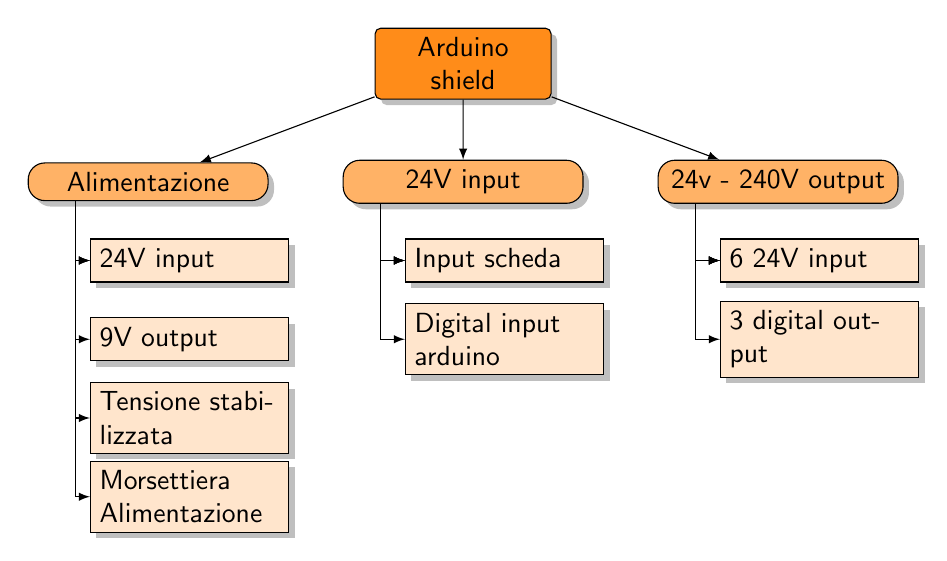
\begin{tikzpicture}[
            level 1/.style={sibling distance=40mm},
            edge from parent/.style={->,draw},
            >=latex]
          
          % root of the the initial tree, level 1
          \node[root] {Arduino shield}
          % The first level, as children of the initial tree
            child {node[level 2] (c1) {Alimentazione}}
            child {node[level 2] (c2) {24V input}}
            child {node[level 2] (c3) {24v - 240V output}};
          
          % The second level, relatively positioned nodes
          \begin{scope}[every node/.style={level 3}]
          \node [below of = c1, xshift=15pt] (c11) {24V input};
          \node [below of = c11] (c12) {9V output};
          \node [below of = c12] (c13) {Tensione stabilizzata};
          \node [below of = c13] (c14) {Morsettiera Alimentazione};
          
          \node [below of = c2, xshift=15pt] (c21) {Input scheda};
          \node [below of = c21] (c22) {Digital input arduino};
          
          
          \node [below of = c3, xshift=15pt] (c31) {6 24V input};
          \node [below of = c31] (c32) {3 digital output};
          \end{scope}
          
          % lines from each level 1 node to every one of its "children"
          \foreach \value in {1,2,3}
            \draw[->] (c1.195) |- (c11);
            \draw[->] (c1.195) |- (c12);
            \draw[->] (c1.195) |- (c13);
            \draw[->] (c1.195) |- (c14);
          
          \foreach \value in {1,...,4}
            \draw[->] (c2.195) |- (c21);
            \draw[->] (c2.195) |- (c22);
          
          \foreach \value in {1,...,5}
            \draw[->] (c3.195) |- (c31);
            \draw[->] (c3.195) |- (c32);

          \end{tikzpicture}
    \end{center}
\end{figure}
\noindent
Tutte e tre le parti vanno ad interfacciarsi con Arduino, dal momento che è lui che gestisce tutto, anche gli output a 240V attraverso lo shield.\\

% =============== allegati ===============
\vfill
\section{allegati} 
\pagenumbering{Roman}
\label{sec:allegati}
\paragraph{Schema progetto}
\href{https://drive.google.com/file/d/1qK_MUvGxWjfc9fLc7l3a6s5mL5L6D6fg/view?usp=sharing}{Link pdf}
\begin{figure}[H]
   \centering
        \includegraphics[scale=0.5]{/home/rib/varie/progetto-ini.pdf}
       \label{prog}
       \caption{Schema iniziale per la progettazione della scheda}
\end{figure}

\paragraph{Schema di multisim}
\href{https://drive.google.com/file/d/1VOPnspiu-4T2ZOR6uaUWNH1DUEd0fUcg/view?usp=sharing}{Link immagine}
\begin{figure}[H]
   \centering
        \includegraphics[scale=0.5]{/home/rib/varie/multisimp-nobkg.png}
       \label{multisim}
       \caption{Schema Multisim con collegamenti fatti}
\end{figure}

\paragraph{Schema di Ultiboard}
\href{https://drive.google.com/file/d/1ZlJ_AIXvgzdlvAawX5noBu48i03zm5dP/view?usp=sharing}{Link immagine}
\begin{figure}[H]
    \centering
        \includegraphics[scale=0.3]{/home/rib/varie/image.png}
        \label{ultiabroad}
        \caption{Schema Ultiboard per la realizzazione del pcb}
\end{figure}

\paragraph{Render 3d}
\href{https://drive.google.com/file/d/1EMIzjUSU50ij58dLTjCctJGQM4YIgIii/view?usp=sharing}{Link immagine}
%\begin{figure}[H]
 %   \centering
  %      \includegraphics[scale=0.5]{/home/rib/varie/3dboard.png}
   %     \label{3d}
%\end{figure}
\subsection{Preventivo componenti}
% ======================================== Tabella ========================================    
    \begin{center}
        \begin{tabular}{| c | c | c | c| c |c|} 
        \hline
        \rowcolor{BurntOrange} Codice prodotto & Dispositivo & Descrizione & Quantità & Prezzo & Totale\\ [0.5ex] 
        \hline
        \rowcolor{Peach} G6E-134P-US & Relè & componente elettromeccanico (output)& 3 & 4 & 12\\
        \hline
        \rowcolor{Apricot} ??? & Dissipatore & dissipatore per LM7809CT & 1 & 2 & 2\\
        \hline
        \rowcolor{Peach} 4N25 & Optoisolatore & controllo di circuiti di potenza & 4 & 0.56 & 2.24\\
        \hline
        \rowcolor{Apricot} SRD-12VDC-S L-C & Transistor  &  transistor elettromeccanico potenza & 3 & 1 & 3\\
        \hline
        \rowcolor{Peach}prova & Led & diodo Led verde & 7 & 0.14 & 0.98\\
        \hline
        \rowcolor{Apricot} 1N6267A & Diodo Zener & stabilizzatore di tensione & 5 & 0.5 & 2.5\\
        \hline
        \rowcolor{Peach} 1N4001G & Diodo & serve a evitare ritorni di corrente & 4 & 0.25 & 1\\
        \hline
        \rowcolor{Apricot} ??? & Resistore 330$\Omega$ & dissipatore di corrente  & 7 & 0.11 & 0.17\\
        \hline
        \rowcolor{Peach} ??? & Resistore 1.5k$\Omega$ & dissipatore di corrente & 8 & 0.14 & 1.12\\
        \hline
        \rowcolor{Apricot} ??? & Resistore 560 $\Omega$ & dissipatore di corrente & 3 & 0.12 & 0.48\\
        \hline
        \rowcolor{Peach} ??? & Resistore 3.3 k$\Omega$ & dissipatore di corrente & 4 & 0.12 & 0.48\\
        \hline
        \rowcolor{Apricot} ??? & Condensatore 10 $\mu$F & condensatore elettrolitico & 1 & 0.15 & 0.15\\
        \hline
        \rowcolor{Peach} ??? & Condensatore 22 $\mu$F & condensatore elettrolitico & 1 & 0.2 & 0.2\\
        \hline
        \rowcolor{Apricot} ??? & Fusibile & protegge dalle sovracorrenti & 1 & 0,7 & 0.7\\
        \hline
        \rowcolor{Peach} LM7809CT & Trasformatore  & Trasformatore di tensione da 24V a 9V & 1 & 0.3 & 0.3\\
        \hline
        \rowcolor{Apricot} ??? & Morsettiera x10 & morsettiere input e output & 2 & 1.4 & 2.8\\
        \hline
        \rowcolor{Peach} ??? & Morsettiera x2 & Alimentazione & 1 & 0.6 & 0.6\\
        \hline
        \rowcolor{Apricot} ??? & Morsettiera x6 & Arduino analog input & 1 & 1 & 1\\
        \hline
        \rowcolor{Peach} ??? & Morsettiera x8 & Connettore alimentazioni e arduino I/O & 2 & 1,3 & 2,6\\
        \hline
   \end{tabular}
   \vskip 2mm
   \begin{tabular}[h]{|p{4cm}| p{3cm}|  }
       \hline
        \rowcolor{BurntOrange} Prezzo totale & \cellcolor{white} \hspace{1cm} 33,84\\ 
        \hline
   \end{tabular}
   \end{center}
%======================================== Fine Tabella ========================================
\vfill
\vskip 4mm 
\section{Bibliografia}
   \label{sec:bibliografia}
   \begin{itemize}
       \item \href{https://datasheetspdf.com/pdf/766811/ThinkiSemiconductor/LM78XX/1}{LM7809CT datasheet}
       \item \href{https://www.alldatasheet.com/datasheet-pdf/pdf/2846/MOTOROLA/4N25.html}{4N25 datasheet}
       \item \href{https://www.alldatasheet.com/datasheet-pdf/pdf/1131947/SONGLERELAY/SRD12VDCSLC.html}{SRD-12VDC-S L-C datasheet}
       \item \href{https://it.farnell.com/on-semiconductor/1n4001g/diodo-standard-1a-do-41/dp/1458986?gclid=CjwKCAjwqcKFBhAhEiwAfEr7zUiXu7byYKAv4I9jzqX1HOrYwDHbs8iKbdpKXM1QnqVZ_xLJMfnMjxoCd9kQAvD_BwE&mckv=s_dc|pcrid|522005845083|kword|1n4001g|match|p|plid||slid||product||pgrid|122762829255|ptaid|kwd-10795764537|&CMP=KNC-GIT-GEN-SKU-MDC-Semiconductors}{1N4001G datasheet}
       \item \href{https://omronfs.omron.com/en_US/ecb/products/pdf/en-g6e.pdf}{G6E-134P-US datasheet}
       \item \href{http://www.farnell.com/datasheets/2240125.pdf}{1N6267A datasheet}
       \item \href{https://www.vincenzov.net/tutorial/stampati/spessorepiste.htm}{dimensionamento piste}
       \item controllo prezzi \begin{itemize}
            \item \href{www.mouser.it}{mouser}
             \item \href{amazon.it}{amazon}
            \item \href{https://www.digikey.com/en/products/detail/omron-electronics-inc-emc-div/G6E-134P-ST-US-DC9/369175}{digikey}
       \end{itemize} 
   \end{itemize}
\end{document}
